\def\year{2015}
%File: formatting-instruction.tex
\documentclass[letterpaper]{article}
\usepackage{aaai}
\usepackage{times}
\usepackage{helvet}
\usepackage{courier}
%%
\usepackage{graphicx}
\usepackage{url}
\usepackage{amsfonts}
\usepackage{moreverb}
%%
\usepackage{bm}
\usepackage{paralist}
%%
% so we don't need to specify figures subdirectory in figure code
\graphicspath{{./figures/}}
\usepackage{subfig}

%needed to change table colors
\usepackage[table]{xcolor}
%%
\frenchspacing
\setlength{\pdfpagewidth}{8.5in}
\setlength{\pdfpageheight}{11in}
\pdfinfo{
/Title (Insert Your Title Here)
/Author (Put All Your Authors Here, Separated by Commas)}
\setcounter{secnumdepth}{0}  
\renewcommand{\arraystretch}{1.2} % General space between rows (1 standard)


 \begin{document}
% The file aaai.sty is the style file for AAAI Press 
% proceedings, working notes, and technical reports.
%
\title{Spoken Dialog Systems for Health Interventions using Fully Autonomous Humanoid Robots}
% \author{{\Large\bf Saminda Abeyruwan} \\ {\Large\bf Andreas Seekircher} \\ {\Large\bf Ubbo Visser}\\
% University of Miami\\
% Department of Computer Science\\
% Coral Gables, FL 33146\\ 
% \{saminda,aseek,visser\}@cs.miami.edu\\
% \And  {\Large\bf Ramesh Baral} \\ {\Large\bf Ugan Yasavur} \\ {\Large\bf Christine Lisetti}\\
% Florida International University\\
% Computing \& Information Sciences\\
% Miami, FL 33199 \\
% \{rbara012,uyasa001,lisetti\}@cis.fiu.edu\\
% }


\maketitle
\begin{abstract}
We integrated a spoken dialog system that we developed to deliver brief health interventions with a 
speech-enabled 3D virtual character with a fully autonomous humanoid robot (NAO). The dialog 
system is based on Markov decision processes (MDPs). We use model free off-policy algorithms in 
reinforcement learning (RL) with the data  collected from real user interactions to obtain the 
(near-) optimal policy. The system begins to learn optimal dialog strategies for initiative 
selection, and for the type of confirmations that it uses during the interaction. The health 
intervention framework, delivered by a 3D character instead of the NAO, has already been evaluated, 
with statistically significant results in terms of task completion, ease of use, and future 
intention to use the system.  The current spoken dialog system for the humanoid robot is a novelty with high potential impact to improve children's health.
\end{abstract}

%Keywords Spoken dialog Systems á Reinforcement Learning á Virtual Agents and Avatars á Behavior
%Change Brief Intervention

\section{Introduction} \label{intro}

%Spoken dialog systems (SDS) and autonomous humanoid robots are emerging fields of research which, {\em together}, could bring a revolution to human-robot interaction as we know it. 
Latest developments in spoken dialog systems (SDS) show complementary progress for the development of  embodied conversational agents (ECA) \cite{YASCLL14}. Yet, very little of
this progress has been used for autonomous humanoid robots, which have also recently demonstrated the ability
to serve in health interventions. The
humanoid robot NAO specifically has been used in a variety of applications in the health domain (e.g.,
\cite{MAJA13}), including user studies which demonstrate the usefulness of the NAO platform.

Dahl and Boulos (2013) \nocite{robotics3010001} gave a recent overview of how {\bf robots are used in
healthcare}. Apart from the  surgical robots that are tele-operated by a human doctor, robots support
the daily work in hospitals, mainly in logistics (e.g., Atheon TUG platform \cite{bloss2011mobile}
or HelpMate \cite{evans1998helpmate}). Several other studies have looked at different autism
spectrum disorders. The main goal is to provide therapy with the help of an intelligent robotic
agent that improves both social and communication skills of the children involved. One example is
the KASPAR robot \cite{robins2012scenarios}. Its creators use robot-based play scenarios that can
be tailored for types of disability and skill areas that need to be motivated. Another example has
been created by Bekele and colleagues. They focus on communication behaviors, in particular
head-tracking to manifest the robots engagement in the on-going interaction \cite{bekele2013step}.  

Several studies involve the {\bf humanoid robot NAO}. Csala and colleagues, for example,
studied the effectiveness of a tele-operated NAO humanoid robot in improving the wellbeing of
children having undergone marrow-transplants. Although there is no conversation with the user
involved, the study demonstrated that the NAO robot is well suited for this task due to its small
size and robustness \cite{Csala2012}. Also, the study identified personalization as a key
requirement for success. The NAO robot has also been used by Belpaeme and colleagues who used the
robot to both entertain and educate children suffering from diabetes in a hospital environment
\cite{belpaeme2012multimodal}. This work is interesting to our approach as it is focused on
providing high levels of robot autonomy using a natural language interface and a long-term memory
structure that allowed children to develop a personal relationship with the robot. Both studies by
Csala and colleagues, and Belpaeme and colleagues, took place in hospitals, and both efforts were
greatly appreciated by the children involved.

{\bf Dialog systems} can be classified into two main categories based on their dialog management 
technique, which can be either based on machine learning, or hand-crafted.  Systems based on RL are 
popular in the SDS community and are reported to work better than hand-crafted ones for  
speech-enabled systems against noisy speech recognition \cite{young2013pomdp}. 
Hand-crafted systems, on the other hand, can be divided into three subcategories, with dialog 
management approaches using: finite states \cite{sutton1998CSLU}, plans and inference rules 
\cite{ferguson1998trips,Bohus2009} or information states \cite{Traum03}. Intelligent robotics agent 
researchers have not yet integrated these results in their dialog systems to our knowledge, and their dialog management usually still relies on 
hand-crafted methods \cite{morbiniFlores2012,Bickmore2010}. 
% BUT BICKMORE AND MORBINI DON'T WORK ON INTELLIGENT ROBOTICS, ONLY 3D CHARS?

In this article, we discuss a new mode of delivery - a spoken dialog system coupled with a NAO robot - 
for health interventions that can help people adopt healthy lifestyles.  The dialog system can 
deliver brief health interventions (BI), which are short, well structured, one-on-one counseling 
sessions, focused on specific aspects of problematic lifestyle behavior (e.g. overeating, poor diet, 
heavy drinking). BIs, which are top ranked out of 87 treatment styles in terms of efficiency 
\cite{miller2002mesa} and which can be delivered in 3-5 minutes \cite{Moyer2002}, assess a person's 
problem behavior, and provide advice about ways to eliminate it. 


\section*{Approach}

In this section, we briefly discuss the approach used to develop the dialog 
agent (see \cite{YASCLL14} for more details). According to the 
clinician's guide for conducting brief interventions from the National Institute on Alcohol Abuse 
and Alcoholism (NIAAA) \cite{national2007helping}, a brief intervention for alcohol-related health 
problems can be delivered in three sequential steps (Figure 
\ref{fig:dialog_manager}): 
\begin{inparaenum}[1)] 
\item {\em Screening} about alcohol {\em use}; 
\item {\em Assessing} for alcohol use disorders in two sequential processes: 
  \begin{inparaenum}[a)] 
    \item assessment of potential alcohol {\em abuse}; and 
    \item assessment  of potential alcohol {\em dependence}
  \end{inparaenum}; 
\item {\em Advising} and assisting the patient according to the degree of alcohol problems which leads to: 
  \begin{inparaenum} 
    \item advice for {\em at-risk} drinkers; 
    \item and advice for drinkers with alcohol use {\em disorder} (e.g. coordinate care with specialist).
  \end{inparaenum} 
\end{inparaenum}

\subsection*{Dialog Structure for Brief Interventions}

The development of our brief intervention content is based on the guide provided by 
NIAAA \cite{national2006niaaa}. The goal of the dialog agent is to deliver alcohol screening and 
brief interventions based on this guide. Each step contains a set of questions. The {\em Screening for Heavy Drinking  Step}
uses 5 questions to assess the user's {\em alcohol use} or consumption.  If the user 
expresses that (s)he is not consuming alcohol, the interaction is  ended gracefully with advice on recommended limits; otherwise, the dialog continues to the {\em Assessing for Alcohol Use Disorders Step}, see (Figure \ref{fig:dialog_manager}).

The {\em Assessing for Alcohol Use Disorders Step} (i.e. assessing {\em abuse} or {\em dependence}) consists of two sequential sub-steps: 
\begin{inparaenum}[1)] 
\item the {\em Assessing Alcohol Abuse} sub-step, which has 4 questions to assess alcohol {\em abuse} indicators (e.g., risk of bodily harm, relationship trouble); one indicator is enough to establish alcohol {\em abuse}.  In either case, the system then moves to: 
\item the {\em Assessing Alcohol Dependence} sub-step, 
%three or more indicators indicate {\em dependence}.\end{inparaenum}
%The {\em Assessing Alcohol Dependence sub-Step} 
which has  7 questions to access the user's potential dependence (e.g., keep drinking despite problems, not able to stick to drinking limits); it is enough to detect 3 dependence indicators to transit to the {\em Advising on Alcohol Use Disorder Step} (i.e. abuse or dependence).  If the system does not detects 3 dependence 
indicators, it transits to the {\em Advising on At-risk Drinking}. 
\end{inparaenum}

Therefore, the dialog system branches to two 
separate steps at the end of the {\em Assessing for Alcohol Use Disorders Step}. In both branches, the system provides information 
to the user related to the assessment performed by the system.  If the system assessed that the user has an alcohol use 
{\em disorder}, it refers the user to treatment with an addiction specialist, and suggests a drinking goal.  If 
the system assessed that the user is 'only' {\em at-risk}, it gauges his or her readiness to change, and provides feedback and 
information about the person's drinking. Therefore in both stages, the system provides factual 
information about the person's drinking and suggested drinking limits, and asks what is the user's 
intention to change with a single question.  In total there can be a maximum of 18 different 
questions in a complete session.   

\begin{figure}[!t] 
\centering 
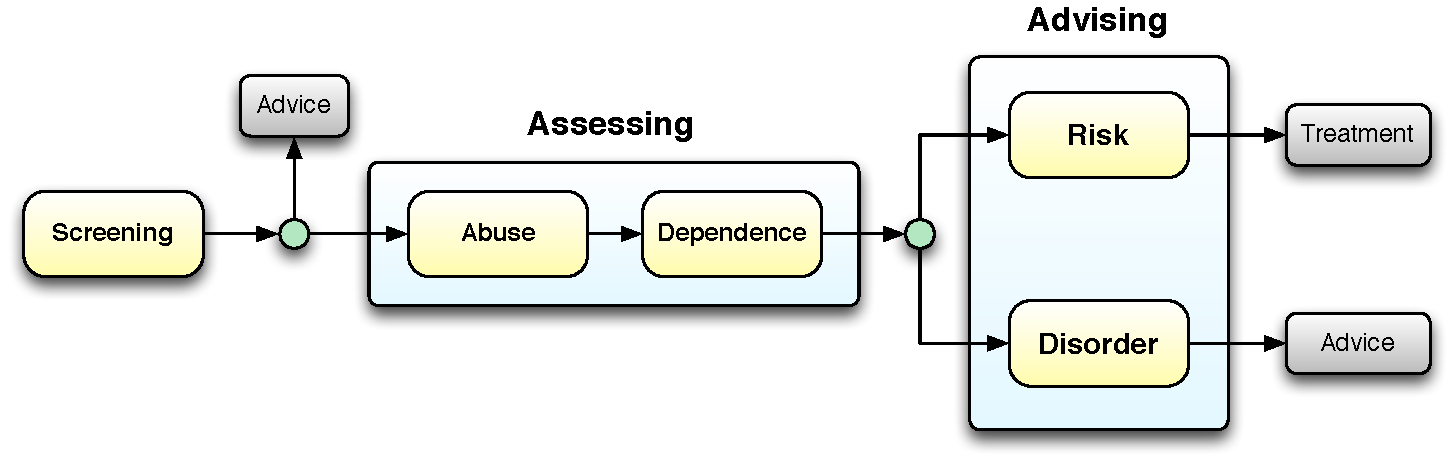
\includegraphics[width=.45\textwidth]{figures/dialog_manager_v2} 
\caption{Dialog structure for brief interventions.} 
\label{fig:dialog_manager} 
\end{figure}

\subsection*{Dialog Agent with Reinforcement Learning}

The goal of the dialog system is to find a (near-) optimal policy that guides the user to an advice 
or a treatment appropriate to the user's alcohol use (the grey boxes in Figure \ref{fig:dialog_manager}) in an efficient manner. 
Model free off-policy algorithms in RL (e.g., Q($\lambda)$ \cite{sutton1998reinforcement}, 
Greedy-GQ($\lambda$) \cite{maei2010toward}, off policy actor-critic \cite{DegrisWS12}) provide the 
means to find (near-) optimal dialog policies by having the agent learn them 
from real experiences, and reward feedbacks. In addition, the RL framework provides many advantages over hand-crafted approaches \cite{lemon2007machine}: \begin{inparaenum}[1)] \item a 
data-driven automatic development cycle; \item provably optimal or near-optimal dialog policies; 
\item  a principled mathematical model for action selection; \item  possibilities for generalization 
to unseen states; and \item reduced development and deployment costs.\end{inparaenum} 

The {\bf Reinforcement Learning framework} is a generalization of MDPs \cite{sutton1998reinforcement}. In oder to develop a RL 
agent, the designer provides the descriptions of the states, actions, and reward functions. As the 
first step, to avoid the data sparsity problem during learning,we
divided  the whole system into 5 RL problems (Figure \ref{fig:5mdpv2}) and learned their 
(near-) optimal policies independently. 

\begin{figure*}[!t]
  \centering    
	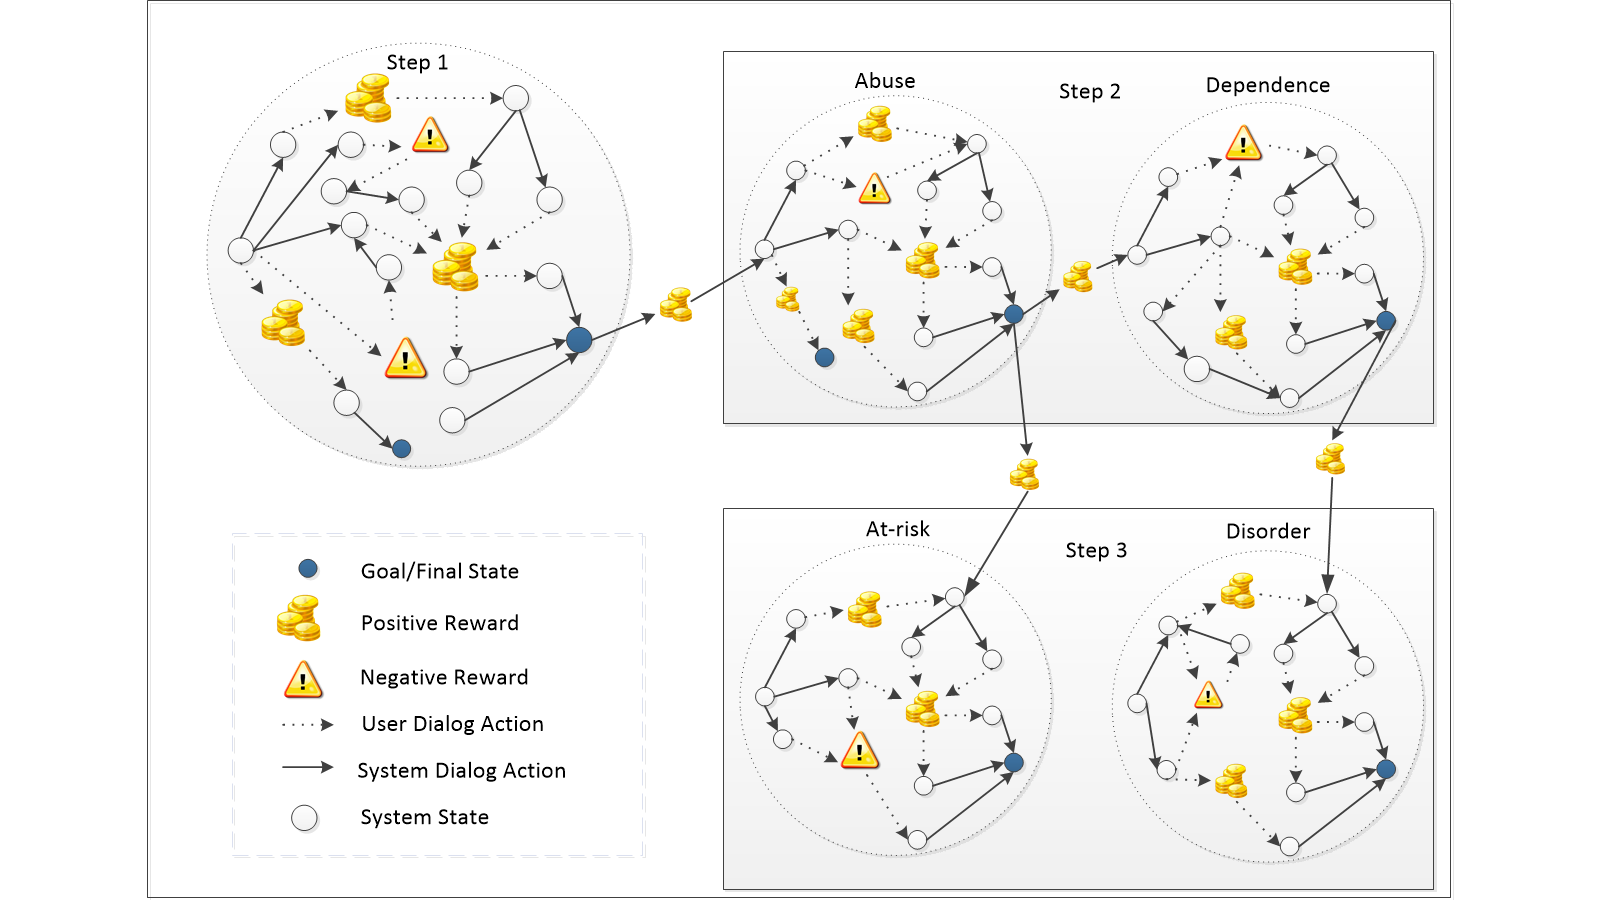
\includegraphics[width=0.9\textwidth]{figures/5MDPV2}
	\caption{Representation of the RL problems.}
  \label{fig:5mdpv2}
\end{figure*}

\begin{table}[!ht]
\caption{State features and its domains for screening about alcohol consumption.}
\label{FeaturesRepresentation}
\begin{tabular}{ | p{14mm} | p{11mm} | p{48mm} | } \hline
    \textbf{Feature} & \textbf{Domain} & \textbf{Description} \\ \hline
    Greeting   & 0,1              & Whether the system has greeted the user. \\ \hline
    Question   & 1,2,3,4          & Which question is being queried.\\ \hline
    Confidence & 0,1,2,3, 4,5,6 & 0,1,2 for low, medium, and high confidence of speech recognizer. 3,4 for
                                  confirmed or not confirmed. 5 to indicate system is waiting for confirmation. 
                                  6 is for to indicate system transit to next question without confirmation.\\ \hline
    Value      & 0,1            & Is the value obtained for current question.\\ \hline
    Grammar    & 0,1            & What type of ASR grammar used, restrictive or dictation (non-restrictive) 
                                  grammar.  \\ \hline
    Auxiliary  & 0,1,2          & Multiple purpose attribute. Use to indicate number of ReAsks and semantic 
                                  valence of the received answer. If it is 0, it indicates, it is not used in 
                                  that state.  \\ \hline
\end{tabular}
\end{table}


A {\em state} is described with 5 features with discrete values (shown in Table 
\ref{FeaturesRepresentation}): \begin{inparaenum}[1)] \item question; 
\item confidence (of speech recognition); \item value; \item grammar; and \item auxiliary. \end{inparaenum} Each 
question is mapped to a possible state. According to our definitions, each question will produce 34 
potential states (some associated states per question have been pruned due to non-reachability). 
Therefore, the dialog agent uses a total of 578 states to represent the states of the environment. Each 
state is associated with 2 actions based on initiative and  confirmation types. The reward 
function is designed to complete each RL problem with the minimum possible number of steps (see \cite{YASCLL14} for details).  

A {\bf rich dialog corpus} that we collected was used during the learning process. The corpus is organized turn by 
turn. Each turn element contains: stage and state information, question asked by the system,  
initiative type,  best speech recognition, grammar type, semantic value or result of the semantic 
parser, N-best recognitions with confidence score, reward gained from the question, cumulative 
reward and sound files. Each XML log file contains sequences of dialog turns for one dialog 
session (Table \ref{sampleDialog} shows  sample dialogs for each stage). The off-policy model free 
Q($\lambda$) algorithm was used to learn a (near-) optimal policy.

\begin{table}[!h]
\caption{Sample Dialogs for each Intervention Step}
\label{sampleDialog}
\begin{tabular}{ p{80mm}  } \hline
    \textbf{Asking about Alcohol Use} \\
    Hello, my name is Doctor House. I am a humanoid robot created to have conversations about 
healthy lifestyle. Today, I am here to talk about drinking to figure out if you have any issues.  
May I ask you few questions about your drinking? \\
\bf{\em{Yes, sure you can.}}\\
Do you sometimes drink beer, wine, or other alcoholic beverages?\\
\bf{\em{Well yes, I drink wine or beer sometimes!}} \\
$\ldots$\\
Ok, thanks for the information you have provided to me about your drinking. Next, I will try to 
determine some important effects of your drinking. \\
    \hline
    \textbf{Assessing for Alcohol Use Disorders} \\
    Have you ever taken risks under the influence, such as drinking and driving, operating a motor 
vehicle, or swimming?\\
\bf{\em{No I have not.}} \\
I see, so you are careful to avoid high risk situations after or while having drinks, right?\\
\bf{\em{Yes, I try to be careful.}} \\
$\ldots$\\
Have you had a period when you spent a lot of time drinking? Or being sick or getting over the bad 
aftereffects of drinking? \\
\bf{\em{Yes several times.}} \\
    \hline
    \textbf{Advising} \\
     Thank you very much for all your answers. Now I'd like to just take one or two more minutes of 
your time. Is that okay? \\
\bf{\em{Yes, please go ahead.}}\\
$\ldots$\\
Thanks for talking with me. I hope you've learned something useful about your drinking pattern.  
Good bye and let's talk again in 3 months! \\
    \hline
\end{tabular}
\end{table}


\section*{Implementation} 

Our implementation is based on two system designs that were 
invented and developed independently in two different research groups. One  
group developed the dialog manager integrated with a 3D virtual 
character.  The system utilizes the user's natural speech as one input parameter and also uses gaze
and non-verbal cues to adapt to the user's social cues. The dialog manager (successfully 
tested with 89 users) operates with five
interconnected MDPs, each representing a step of the intervention \cite{YASCLL14}. The dialog 
manager uses domain specific dialog phrases, with a tailored semantic parser, and a RL agent that 
learns over time how to address and answer the user. 

\begin{figure}[!t] 
\centering 
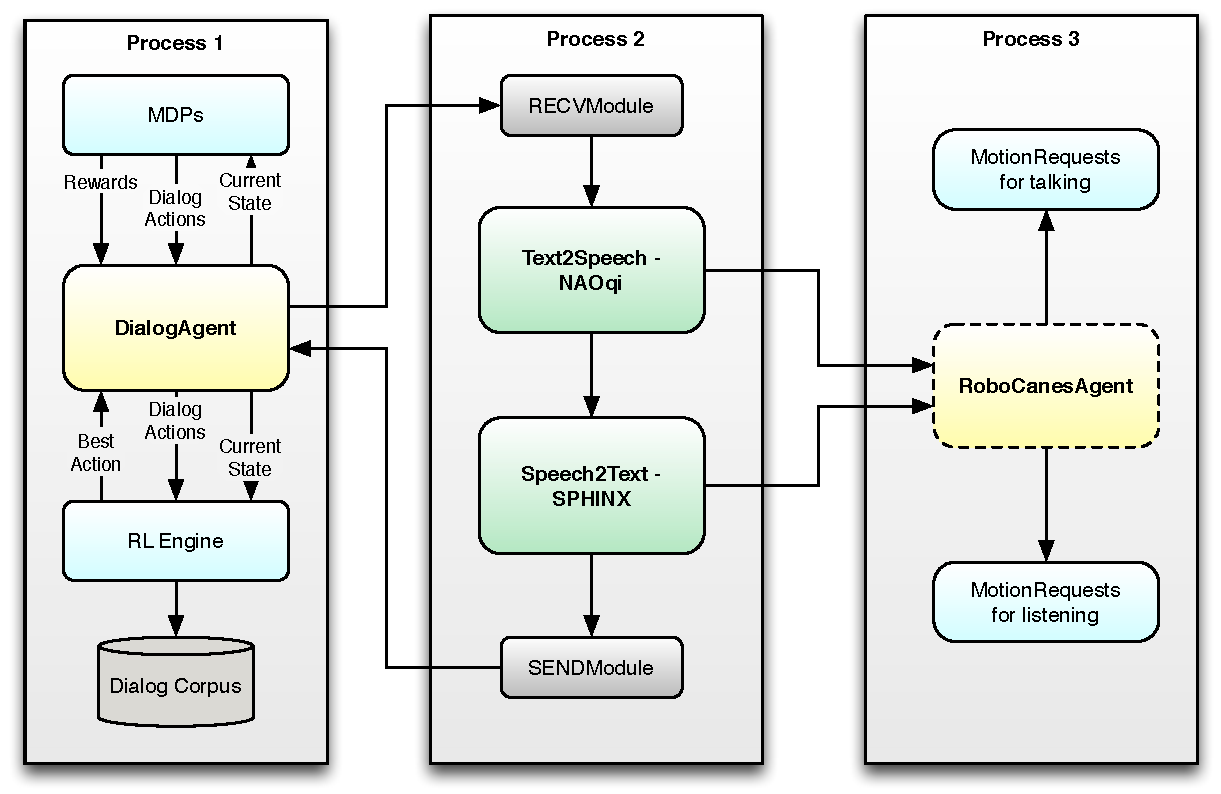
\includegraphics[width=.46\textwidth]{figures/system} 
\caption{System Architecture: {\em Process 1} is the dialog manager; {\em Process 2} delivers the 
robot's spoken utterances and the recognized human's utterances; and {\em Process 3} senses the 
human's non-verbal cues, and controls the robot's motions for appropriate gestures during the 
robot's speech and listening time (e.g. tracks user's face and, if user moves, moves to maintain 
facing position.)} 
\label{fig:system} 
\end{figure}

The backbone of the system described in this article was developed by one of our 
labs,\footnote{We anonymized.} for both simulated and
physical robotic agents that act in dynamic, adversarial, and real-time environments.    
%The group uses the RoboCup domain as an area of investigation. 
%We focus on the  agent's
%actions/behavior to make its own decisions. 
%(for the own team agents). 
The group has developed a fully implemented software system  using NAO robots that not 
only move and walk autonomously in a given environment but 
also communicate in real time with other NAOs. The 
software is stable and
robust and is now integrated with the dialog manager.

The software runs as a single process. The
dialog manager is connected to another process on the robot that makes use of Google speech API 
version 2. 
%The original dialog system described in \cite{YASCLL14} has a language model and grammars, which we plan to  adapt to execute the functions more efficiently on the NAO robot. 
A third process is 
the agent software that can be connected to the dialog. Figure \ref{fig:system} gives an 
overview of the architecture and the three processes. {\em Process 1} is connected to {\em Process 2} using 
Java JNI interface.  The NAO robot then uses NAOqi for the Text-To-Speech 
generation, although we have also implemented and tested other systems such as Festival 
\cite{taylor1998architecture} or eSpeak \cite{eSpeak}, which  also work. {\em Process 2} then makes 
use of the lab agent framework which is responsible for robot motions and 
for the image processing and the audio feedback (no feedback from cameras at the moment yet). The 
robot then uses Google speech API, turns the audio signal into text and sends it back to the dialog 
manager. {\em Process 3} is responsible for coordinating the robot's gestures with its spoken utterances, and uses face tracking to physically follow the user.  The timing between Processes 1 and 2 are based on turns, whereas Process 3 runs with 100 Hz for the 
joint requests and 30 Hz for both cameras.

\section*{Dialog System Evaluation}

Evaluating dialog systems requires two types of evaluation: 1) {\em objective evaluation} of the system performance per se (e.g. task metrics such as task completion, and dialog metrics such average length of the dialog); and 2) {\em subjective evaluation} of the user's experience (e.g. ease of use of the system, intention to reuse the system).

Because the only difference between the current robot-based dialog system and the 3D character-based dialog system \cite{YASCLL14} is that the former uses the Google speech recognition whereas the latter uses the Microsoft speech recognition engine, the results of performance of the dialog system (when it is delivered by the 3D virtual character) provide an indication of what can be expected of the performance of the same dialog system when it is delivered by the NAO.  As discussed in the Conclusion and Future Work Section, our next step will be to use the exact same procedure as the one described below, to evaluate the robot-based dialog intervention.

{\bf Participants.} For the evaluation of the system delivered by the 3D virtual character, 89 subjects were recruited from volunteer university students through fliers and emails.  From 89 participants, 62 of them were males and 27 of them were females; 51 of them were native speakers and 38 of them were non-native speakers,   which realistically represents the diversity of the population in the Miami, Florida area.

University students represents a very appropriate sample for target population for brief interventions. The latest report of NIAAA on college drinking indicated that alcohol problems are very prevalent among college students \cite{NIAAA2007colleges}, and 19\% of college students (ages 18-24) meet the criteria for alcohol abuse or dependence\footnote{From the Diagnostic and Statistical Manual of Mental Disorders, Fourth Edition (DSM–IV), American Psychiatric Association.}. The use of brief interventions with college students to educate students about drinking and  increase their awareness is very common \cite{NIAAA2007colleges}. As a result of many studies, the NIAAA report on college drinking emphasized that ``increased alcohol screening and brief interventions are feasible  and appropriate for identifying and addressing harmful drinking among college students". 

{\bf Procedure.} Participants sat in front of a PC computer running the systems (some the training system and some the testing system as described below), and responded in English to the questions asked by the embodied conversational agent.  The computer was equipped with a USB sound card and a Sennheiser ME 3-ew microphone.

It is important to note that we did {\em not} perform any user training nor speaker adaptation for speech recognition. 

After obtaining an oral consent approved by the University Internal Review Board, we gave the following instructions to each subject before using the system for both experiments:
\begin{compactitem}
\item You will be asked questions about your drinking behavior with an avatar/virtual character.  You may or may not have any alcohol related problems, but we just want you to role-play a person who is having drinking-related problems and give relevant answers to each question.
\item Try to speak clearly and loudly enough.
\item Wait until the avatar stops speaking before you answer.\\
\end{compactitem} 
 \begin{figure}
 \centering
 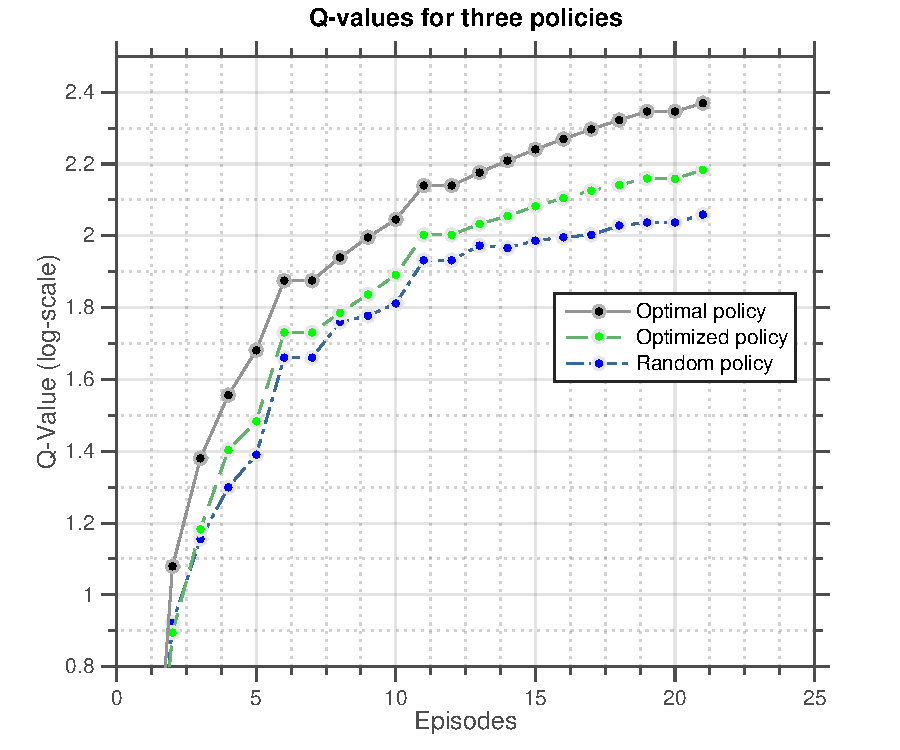
\includegraphics[width=\columnwidth]{figures/q-values.pdf}
 \caption{Q-values for each episode, the X-axis shows the number of episodes and the Y-axis shows the log-scale Q-values.}
 \label{q-values}
 \end{figure}



{\bf Objective Evaluation.}  
%SAM: CAN YOU EXPLAIN BRIEFLY HOW Q-VALUES ARE ABLE TO SUMMARIZE THE RESULTS NICELY?
As shown in Figure \ref{q-values}, we compared Q-values for each episode. An episode can be defined as completing one question and passing to the next question. It is important to note that completion of one question does not mean that the system obtained the information it was trying to get. It is possible for the system to transit to the next question without having obtained the information, and in that case, the system receives negative reward. 
%We described the details of the reward function in Section \ref{Reward}. 
We show the improvement of Q-values for each episode in Figure \ref{q-values}. We have  21 episodes because we have 18 questions, plus transitions between MDPs. As shown in Figure \ref{q-values}, the optimized policy performed better, even though it is not optimal. We have to note that \textit{optimal policy} represents the highest reward that the system can achieve, whereas the \textit{random policy} and the \textit{optimized policy} represent the average score that the system collected in training and testing operation modes, respectively.\\


{\bf Subjective Evaluation}. After the subjects completed the intervention, the subjects answered a survey aimed at evaluating the user's experience with the system. 
%The survey has two parts, the first part has 4 yes/no questions and the second part is a 34-item questionnaire about the subject's assessment and experience with the system. 

%In the first part, 
We asked questions about reuse ``Would you use the system in future?", and ease of use ``Is the system easy to use and is it easy to understand how to use the system?", and ``Did the system understood what you said" and ``Did you know what to say to the system in each turn".

Our evaluation of the subjective aspects  
%shown in Figure \ref{yesNoEva} 
demonstrated that acceptability of the system by users is very high in terms of {\em Ease of Use} (81 yes / 8 no), and {\em Intention to Reuse} (63 yes / 26 no)
% DISCUSS ACTUAL NUMBERS, ADD UNIT IN FIGURE FOR Y AXIS, SAME FOR OTHER FIG BY THE WAY)
% NOT CLEAR HOW INTENTION TO REUSE WAS EVALUATED THOUGH, WHAT QUESTION(S)?
the system. The answers to {\em What to say to system?} revealed that sometimes users do not know how to answer the system questions: it might be that when in user initiative mode, i.e. when the system asks open questions, users may not be sure to what extend they can provide details. This suggests the need for the agent to initially brief the user about its language understanding abilities at the beginning of the conversation.
% DISCUSS: WHY DO YOU THINK THAT IS?  THE QUESTIONS WERE PRETTY SIMPLE, WHY DIDN'T THEY KNOW HOW TO ANSWER?
The {\em System understood} criterion indicated that most of the users think that the system understood what they said.  This suggests that the system ample use of confirmation questions when it is unsure it understood, helps reassure users they have been understood.

\begin{figure}
 \centering
 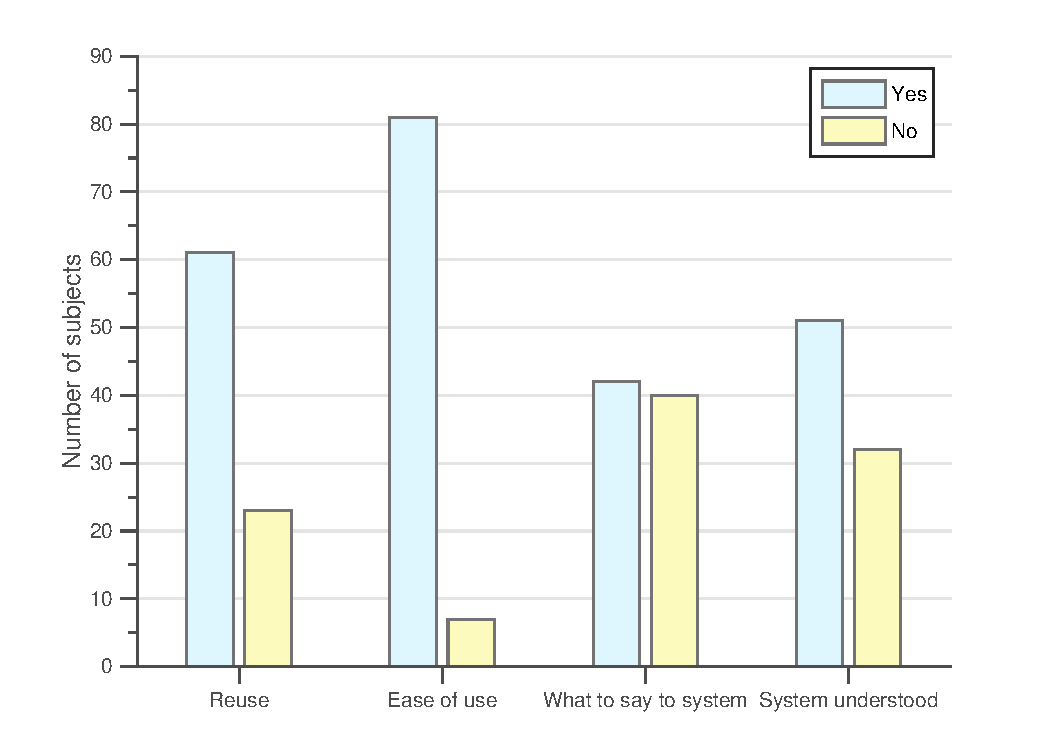
\includegraphics[width=\columnwidth]{figures/subjective.pdf}
 \caption{Subjective Evaluation}
 \label{yesNoEva}
 \end{figure}
 
%In the second part of the subjective assessment, we used a 34-item questionnaire named {\em Subjective Assessment of System Speech Interfaces (SASSI)} \cite{SASSI}. It is a widely used evaluation questionnaire in the SDS community. The subjects answered a randomized list of SASSI questionnaire on a 7-point Likert scale. The SASSI questionnaire queries 6 aspects of the user's assessment and experience with the system.  These aspects are \textit{Accuracy}, \textit{Likeability}, \textit{Cognitive Demand}, \textit{Annoyance}, \textit{Habitability}, and \textit{Speed} of the system. 

\section*{Conclusion and Future Work} 

We have implemented a computerized brief intervention that can be delivered by a speech-enabled 3D virtual character and a NAO robot.  We anticipate that the positive results of the speech-enabled 3D character delivering the intervention will be reproduced when we next evaluate the NAO delivering the intervention.

Furthermore, brief interventions have a single and simple structure that can be adapted to a variety of target behaviors, such as poor diet, overeating, or lack of exercise, among others \cite{Moyer2002}.
The appeal of the NAO to children 
\cite{belpaeme2012multimodal} makes it particularly suitable to become a child's favorite health 
coach, say, to discuss eating more fruits and vegetables on a daily basis. Our NAO platform 
provides additional advantages such the ability to physically demonstrate physical exercises, when the target behavior of the brief intervention is lack of exercise.

\bibliographystyle{aaai}       
\bibliography{library}   


\end{document}
